\section{Numerical illustration}\label{sec:numerics}
The script \texttt{experiments/generate\_convergence.py} computes 21 binary64
Newton iterates and 21 bisection midpoints. At index zero the Newton value is
$2$ and the bisection value is the midpoint $1.5$ of $[1,2]$. After each
midpoint evaluation, the sign of $x^2-2$ determines which half interval is
retained. In exact arithmetic the interval length before index $n$ is $2^{-n}$,
so its midpoint error is at most $2^{-n-1}$. Equal indices are not equal-cost
comparisons: Newton requires a division while bisection evaluates a sign.

\begin{table}[ht]
\centering
\begin{tabular}{rrrrr}
\toprule
$n$ & Newton & Newton error & Bisection & Bisection error \\
\midrule
0 & 2.0000000000 & 5.858e-01 & 1.5000000000 & 8.579e-02 \\
1 & 1.5000000000 & 8.579e-02 & 1.2500000000 & 1.642e-01 \\
2 & 1.4166666667 & 2.453e-03 & 1.3750000000 & 3.921e-02 \\
3 & 1.4142156863 & 2.124e-06 & 1.4375000000 & 2.329e-02 \\
4 & 1.4142135624 & 1.595e-12 & 1.4062500000 & 7.964e-03 \\
5 & 1.4142135624 & 1.254e-16 & 1.4218750000 & 7.661e-03 \\
\bottomrule
\end{tabular}

\caption{Initial computed iterates and absolute errors (rounded).}\label{tab:iterates}
\end{table}
\begin{figure}[ht]
\centering
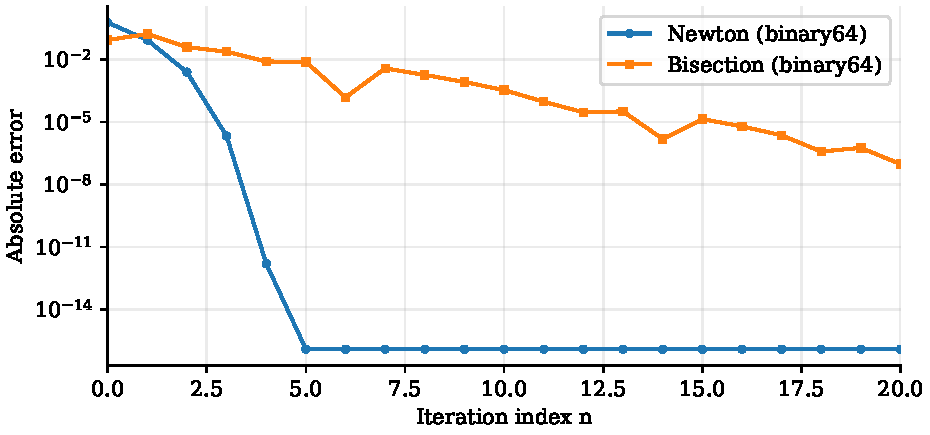
\includegraphics[width=.85\linewidth]{figures/convergence.pdf}
\caption{Computed absolute errors on a logarithmic vertical axis.}
\label{fig:convergence}
\end{figure}

Errors are measured against an 80-digit decimal evaluation of $\rtwo$, using
the exact decimal representation of each computed binary64 value. This avoids
mistaking equality with a rounded binary64 reference for exact accuracy.
For plotting only, errors smaller than $10^{-18}$ are clipped to $10^{-18}$;
the CSV retains the measured errors. The finite reference precision is far
below the scale of this experiment. Newton reaches a rounding plateau near
$10^{-16}$ while bisection continues a slower reduction over these indices.
Neither the observed speed nor the plateau proves the theorem. They illustrate
the exact analysis and the limitations of its floating-point realization.
